\documentclass[12pt]{article}
\usepackage{graphicx} % For including images
\usepackage[margin=1in]{geometry} % For setting page margins
\usepackage{amsmath} % For extended mathematical formatting
\usepackage{fancyhdr} % For custom headers and footers
\usepackage{float} 
\usepackage{subcaption} % Updated to use subcaption instead of subfigure
\setlength{\headheight}{15pt} % Adjust headheight as recommended
\pagestyle{fancy}
\fancyhf{}
\rhead{EE569 Digital Image Processing}
\lhead{HOMEWORK \#5}
\rfoot{Page \thepage}
\usepackage{enumitem}
\setlist[itemize]{font=\bfseries} 
\begin{document}
	
	\begin{center}
		\Large
		\textbf{Homework \#6}
		
		\vspace{0.2cm}
		\normalsize
		Issued: 03/28/2024 \hfill Due: 05/01/2024
	\end{center}
\section*{Problem 1: Origin of Green Learning (GL)}
\subsection*{(a) Feedforward-designed Convolutional Neural Networks (FF-CNNs)}
	\begin{figure}[H]
		\centering
		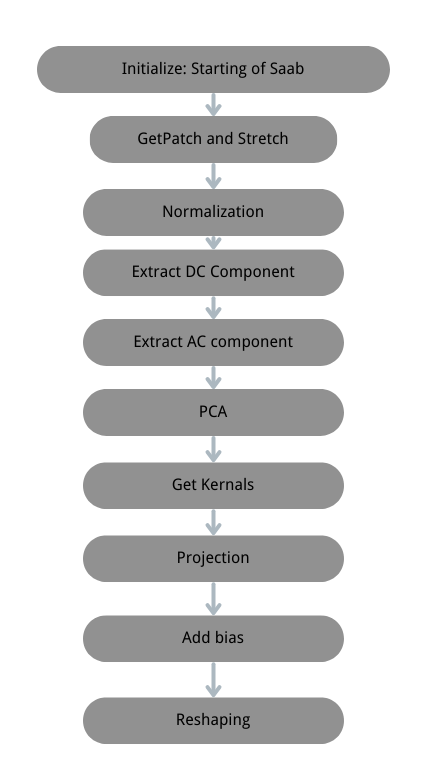
\includegraphics[width=0.6\textwidth]{saab.png}
	\caption{Saab Process}
	\label{p1a}
\end{figure}
	(1) As shown in fig\ref{p1a}, the saab process is a transformed way of PCA. In the start of the Saab Process, the data is applied by getPatch and stretch. Then the process tries to calculates DC, then minus all other anchors by DC to get the AC. After getting the component of x on ac directions, PCA is applied to reduce dimension. Then, get the kernals, and using the largest norm to projection. Then bias are added to the data. Following is the reshaping process, then goes to output. 
	\\
	(2) Similarities and Differences between FF-CNN and BP-CNN:\\
	\begin{itemize}
		\item Similarities: Both types of CNN have a similar archetecture, and both of them are classification models. Both model uses neurons, convergence layers, pooling layers, fully connected layers and output layers. 
		
		\item Differences: BP-CNN trains its parameters in each layer by a large number of iterations, working along with multiple neurons in calculation. However, FF-CNN is a one-pass system, which means it could just use statistics from last layer, using unsupervised learning in feature extraction to get the parameters. By the way, FF-CNN add a bias term to output feature map, which could improve the efficiency of PCA's simplifying process. In the classification step in FF-CNN, it adapts various subclassifications within a main class, offering more precise classification .
		
		\item Advantages: Thanks to FF-CNN's unique features in subclassification, it has much higher accuracy than ordianry BP-CNNs. Also, because it avoids many iterations by adapting one-pass parametering, it is much faster and takes fewer memory when working. 
				

	\end{itemize}
\subsection*{(b) Understanding PixelHop and PixelHop++}
	(1) SSL methodology is a computationally efficient method in maching learning. Instead of old models using only supervised BP process, it takes unsupervised learning method inclduing K-means. This could improve its efficiency of computation, and makes it less rely on the size of the training dataset. 
	\\\\
	(2) The first Module of SSL is extracting features from the input data. The modules uses methods including PCA to reduce dimennsions of the data without applying any labels\\
	The second module involves aggregating the features to capture more complex structures in the data. It extracts statistical values to enhance the feature maps's features.\\
	The third module is used for final classification. \\\\
	(3) Neighbourhood construction gathers the information on pixels in a window, reshaping the data to get additional information. Pixelhop applying saab transform in subspace approximation, while Pixelhop++ applies channel-wise Saab in this step.\\
	Saab processes the whole feature map, extracting pathces from all over the map, and apply PCA to comput the anchor vectors.\\
	 Comparing to saab, cwSaab applies the Saab transform channel-wise, which means transform is applied separately to each channel of the input data or feature maps. It provides a more granular approach by processing each channel independently, which can lead to more tailored and potentially more effective feature extraction. It adds a THE 1 and THE2 to decide whether to keep the channel as leaf nodes or discarding them. 
	\section*{Problem 2: PixelHop \& PixelHop++ for Image Classification}
	 \subsection*{(a) Building PixelHop++ Model}
	 \subsection*{(b) Comparison between PixelHop and PixelHop++}
	 The table of details of trainning of PixelHop and PixelHop++ on MINST and Fashion MINST is listed in the table below in \ref{p1a}.
	 \begin{table}
	 	\begin{tabular}{|c|c|c|}
	 		\hline  KDE for both Models&DSM&EBM\\
	 		\hline Checker&-3.9906778289257354&-8.537413285032038\\
	 		\hline Gaussian&-1.6150337910237458&-12.094435571973383\\
	 		\hline Spiral&-74.80091074585938&-19.91811519787057\\
	 		\hline PinWheel&-1.0175161906712928&-12.477515766573315\\
	 		\hline
	 	\end{tabular}
	 \end{table}
	 \subsection*{(c) Error analysis}
\end{document}